\section{Summary} \label{chapter6:summary}

This thesis presented an equivalence between the event-driven execution model and the pipeline execution model.
This equivalence was implemented into two compilers.
The first compiler allows to identify the rupture point to form chains of stages from programs targeting the event-driven execution model.
The resulting chains still depends on a common memory store.
The second compiler, stemming from the first one, identifies the entry points of these chains - start rupture points - and enforces isolation to form a parallel pipeline.

With these two contributions, it is possible to transform the modular representation of an application into a pipeline representation.
The modular representation allows development productivity, while the pipeline representation executes efficiently.
A development team shall then use these two representations to continuously iterate over the implementation of an application, and reach the best compromise between productivity and efficiency.

The next paragraphs summarizes the two execution models, and the steps of this equivalence from one model to the other.

\subsection{Models} \label{chapter7:summary:model}

\paragraph{Event-driven execution model}

The event-driven execution model is targeted by productive programming languages.
It processes a queue of asynchronous events by scheduling handlers cooperatively.
Each handler can asynchronously request resources and define handlers to receive the resource response. 
The handlers are chained by these asynchronous requests using continuation passing style.
Apart from the resource response, the communication between tow handlers is done via closures.
The downstream handler gets access to the environment of its creation through a closure.

They are organized similarly to a pipeline, each handler being a stage, with the data flowing from one stage to the other.
However, the handlers still share a common memory store.
It allows the higher-order programming required for productivity.
But it also avoids the parallelism required for efficiency.

\begin{figure}
  \centering
  \textfig{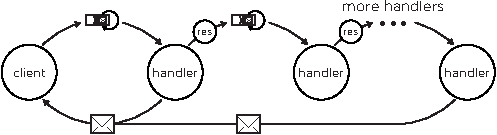
\includegraphics[width=0.8\linewidth]{../resources/cont-chain.pdf}}
\end{figure}

\paragraph{Fluxional execution model}

The fluxional execution model is targeted by a more efficient programming language.
It executes an application expressed as a network of independent application parts called fluxions.
The fluxions communicate by messages, and form a pipeline similarly to the handlers of the event-driven execution model.
They are executed in parallel to distribute the computation across several cores and increase the performance efficiency.
They rely on isolated memory store, called context to allow this parallel execution.
When several fluxions need to rely on the same memory store, they are grouped, and executed sequentially.
When they are independent, they are isolated to increase performance efficiency.

The similarity between the event-driven execution model and the fluxional execution model leads to the equivalence presented in the next paragraph.
With this equivalence, the versatility of fluxions allows to progressively adapt the implementation from a productive, single event-loop, toward an efficient pipeline.

\subsection{Equivalence}

The equivalence describes the transformation from an application targeting the event-driven execution model to execute them in parallel in the fluxional execution model.
This transformation involves two steps: the extraction and isolation of the stages to form the pipeline.

\paragraph{Stage Extraction} \label{chapter7:summary:extraction}

The first step is the identification and extraction of the stages.
The equivalence identifies rupture points between stages.
A rupture point is an asynchronous call without subsequent synchronization with the caller.
It indicates a rupture in the synchronous control-flow, and the boundaries between two handlers.
The upstream handler is the one calling the asynchronous call, the downstream handler is the callback provided to the asynchronous call.

There are two kinds of rupture points: \textit{start} and \textit{post}.
\textit{Start} rupture points directly receives the input stream, and start the execution of the chain of stages for each new datum in the stream.
\textit{Post} rupture points indicates a continuity in the chain of stages.

The difficulty in this compilation step is to identify the asynchronous functions indicating the stages.
Because of the dynamic behaviors of Javascript, it is impossible to statically detect these functions.
The compiler implemented from the equivalence is currently unable to reliably detect them.
Instead the compiler rely on the developer to provide a list of asynchronous function names to extract.

\paragraph{Stage Isolation} \label{chapter7:summary:isolation}

% After the extraction of this pipeline,
The second step is the identification of the memory interdependencies between stages.
It intends to isolate the stages so they can be executed in parallel.
The common memory is replaced by message-passing, following some rules to preserve consistency.
\begin{itemize}
\item If a stage needs to hold a variable from one request to the other, this variable is stored in its context.
\item If a downstream stage needs to read a variable from an upstream stage, the variable is sent as part of the message communication.
\item If two stages needs to share a variable, they are grouped on the same execution node to safely share parts of their context.
Their executions are not parallelized to avoid conflicting accesses.
\end{itemize}

The difficulty in this step is to identify the memory dependencies between stages.
The dynamic behaviors of Javascript, it is impossible to statically identify the aliasing in the memory.
The compiler implemented from the equivalence is currently unable identify these interdependencies.
It relies on manual manipulations to complete the transformation.

\separator

These difficulties are details in further details in the next section.
It then presents some perspectives to overcome these limitations.